% Shared preamble of the solution sheets (included by lecture01.tex, lecture02.tex, ...)
\documentclass[11pt, a4paper]{article}
\usepackage[T1]{fontenc}
\usepackage{lmodern}
\usepackage[margin=25mm]{geometry}
\usepackage{amsmath, amssymb, mathtools}
\usepackage{microtype}
\usepackage{parskip}
\usepackage{booktabs}
\usepackage{xcolor}
\usepackage{tikz}
\usetikzlibrary{patterns}
\usepackage{pgfplots}
\pgfplotsset{compat=1.18}
\usepackage{listings}
\usepackage[hidelinks]{hyperref}

% colours of the slides: Dirichlet blue, Neumann orange
\definecolor{dir}{HTML}{2A78D6}
\definecolor{neu}{HTML}{EB6834}
\definecolor{ink}{HTML}{1D2433}
\definecolor{ink2}{HTML}{52514E}
\definecolor{hair}{HTML}{C3C2B7}
\definecolor{codebg}{HTML}{F3F2EE}
\definecolor{water}{HTML}{E3EEF5}

\lstset{language=Python, basicstyle=\ttfamily\footnotesize, breaklines=true,
  postbreak=\mbox{\textcolor{ink2}{$\hookrightarrow$}\space}, keywordstyle=\color{ink}\bfseries,
  commentstyle=\color{ink2}\itshape, stringstyle=\color{ink2}, backgroundcolor=\color{codebg},
  frame=none, xleftmargin=6pt, xrightmargin=6pt, aboveskip=8pt, belowskip=8pt, columns=fullflexible,
  keepspaces=true, showstringspaces=false, upquote=true}

\setlength{\parskip}{0.6em}
\newcommand{\sheet}[2]{%
  {\small\color{ink2}\textsc{Applied math notes}}\par\vspace{-0.4em}
  {\LARGE\bfseries Lecture #1: #2}\par\vspace{0.1em}
  {\large Solutions to the exercises}\par\vspace{0.6em}}
\newcommand{\exercise}[1]{\section*{#1}}
\newcommand{\task}[1]{\par\medskip\noindent\textbf{#1}\quad}


\begin{document}
\sheet{1}{The Galerkin method}

%% ====================================================================== Exercise 1
\exercise{Exercise 1: Analytical solution and error norm for problem 2}

Problem 2: $-u'' = 1$ on $(0, 1)$, $u(0) = 0$, $u'(1) = 0$.

\task{1.} Integrating $u'' = -1$ twice gives $u' = -x + C_1$ and $u = -\tfrac12 x^2 + C_1 x + C_2$. The boundary
conditions give $u'(1) = -1 + C_1 = 0$, so $C_1 = 1$, and $u(0) = C_2 = 0$:
\[
  u(x) = x - \tfrac12 x^2 .
\]

\task{2.} The FEniCS script below (20 elements, as in the notebook) solves the problem with Lagrange elements of degree
1, 2 and 3. For degree 1 the nodal values of $u_h$ agree with $u$ up to round-off, $\max_i |u(x_i) - u_h(x_i)| =
1.1 \cdot 10^{-14}$: \textbf{the FEM solution is exact at the nodes.}

Reason: the error $e = u - u_h$ satisfies $a(e, v_h) = 0$ for all $v_h \in V_h$ (Galerkin orthogonality). With the
hat function $v_h = h_i$, whose derivative is $\pm 1/h$ on the two elements around node $i$,
\[
  \int_0^1 e'\, h_i' \, dx = \frac1h \big(e(x_i) - e(x_{i-1})\big) - \frac1h \big(e(x_{i+1}) - e(x_i)\big) = 0 ,
\]
i.e.\ $-e_{i-1} + 2 e_i - e_{i+1} = 0$ for the nodal errors; at the Neumann end $e_N - e_{N-1} = 0$, and $e_0 = 0$.
Hence $e_i = 0$ at all nodes. (This holds in 1D for this operator, not in general.)

Between the nodes $u_h$ is therefore the linear interpolant of $u$. On an element $[x_{i-1}, x_i]$ the error vanishes
at both ends and has $e'' = u'' = -1$, so
\[
  e(x) = \tfrac12\, (x - x_{i-1})\, (x_i - x), \qquad \max e = \frac{h^2}{8} = 3.1 \cdot 10^{-4} \quad (h = 1/20),
\]
a parabola on every element:

\begin{center}
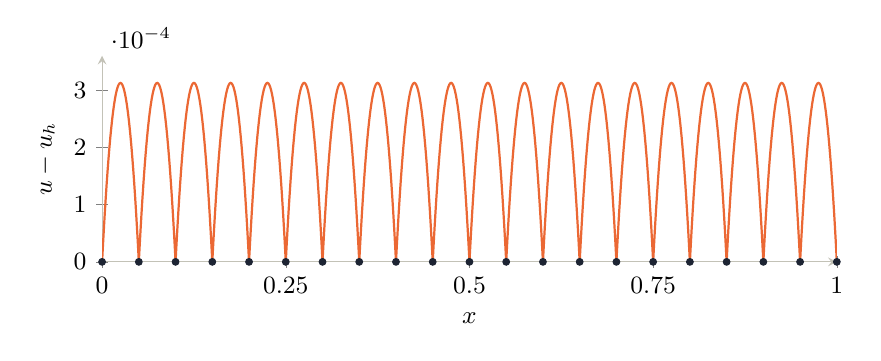
\begin{tikzpicture}
\begin{axis}[width=0.9\textwidth, height=4.2cm, xmin=0, xmax=1, ymin=0, ymax=3.6e-4, xlabel={$x$},
  ylabel={$u - u_h$}, axis lines=left, tick label style={font=\small}, scaled y ticks=base 10:4,
  ytick={0, 1e-4, 2e-4, 3e-4}, xtick={0, 0.25, 0.5, 0.75, 1}, axis line style={hair}, every axis label/.style={font=\small}]
  \addplot[domain=0:1, samples=801, thick, color=neu]
    {0.5*(x - 0.05*floor(x/0.05 + 1e-9))*(0.05 - (x - 0.05*floor(x/0.05 + 1e-9)))};
  \addplot[only marks, mark=*, mark size=1.2pt, color=ink, samples at={0,0.05,...,1}] {0};
\end{axis}
\end{tikzpicture}
\end{center}

\task{3.} With $s = x - x_{i-1}$ and $\int_0^h s^2 (h - s)^2 \, ds = h^5 / 30$, summed over the $N = 1/h$ elements,
\[
  \|u - u_h\|_{L^2}^2 = N \cdot \frac14 \cdot \frac{h^5}{30} = \frac{h^4}{120},
  \qquad \|u - u_h\|_{L^2} = \frac{h^2}{\sqrt{120}} = 2.282 \cdot 10^{-4} \quad (h = 1/20) .
\]
FEniCS gives the same value with \lstinline|errornorm(u_exact, uh, 'L2')|. The error is $O(h^2)$: halving $h$ quarters it.

\task{4.} Results of the script:

\begin{center}
\begin{tabular}{lcc}
  \toprule
  degree & max.\ nodal error & $\|u - u_h\|_{L^2}$ \\
  \midrule
  1 & $1.1 \cdot 10^{-14}$ & $2.282 \cdot 10^{-4}$ \\
  2 & $1.6 \cdot 10^{-13}$ & $1.1 \cdot 10^{-13}$ \\
  3 & $7.1 \cdot 10^{-13}$ & $5.1 \cdot 10^{-13}$ \\
  \bottomrule
\end{tabular}
\end{center}

From degree 2 on the error is round-off. The exact solution $u = x - \tfrac12 x^2$ is a quadratic polynomial, so it
lies in $V_h$ for degree $\ge 2$, and the Galerkin method reproduces any solution that lies in $V_h$: $u_h = u$.

\lstinputlisting{lecture01_exercise1.py}

%% ====================================================================== Exercise 2
\exercise{Exercise 2: Biharmonic equation (theory)}

$A u = u'''' = f$ on $\Omega = (0, 1)$.

\task{1.} The highest derivative is the fourth: $O(A) = 4 = 2s$, so $s = 2$ and $m = s - 1 = 1$.

\task{2.} Integral form and two integrations by parts:
\[
  (Au, v) = \int_0^1 u''''\, v \, dx
  = \big[u'''\, v\big]_0^1 - \int_0^1 u'''\, v' \, dx
  = \big[u'''\, v - u''\, v'\big]_0^1 + \int_0^1 u''\, v'' \, dx .
\]
Variational formulation:
\[
  \int_0^1 u''\, v'' \, dx + \big[u'''\, v - u''\, v'\big]_0^1 = \int_0^1 f\, v \, dx \qquad \text{for all } v .
\]
Boundary terms at $x = 0$ and $x = 1$: $u'''\, v$ (shear force times deflection) and $u''\, v'$ (bending moment times
slope).

\task{3.} With $m = 1$:

\begin{center}
\begin{tabular}{llll}
  \toprule
  prescribed & $c$ & type & condition on $v$ \\
  \midrule
  $u$ (deflection) & 0 & \textcolor{dir}{Dirichlet (essential)} & $v = 0$ there \\
  $u'$ (slope) & 1 & \textcolor{dir}{Dirichlet (essential)} & $v' = 0$ there \\
  $u''$ (bending moment) & 2 & \textcolor{neu}{Neumann (natural)} & none \\
  $u'''$ (shear force) & 3 & \textcolor{neu}{Neumann (natural)} & none \\
  \bottomrule
\end{tabular}
\end{center}

Where $u$ or $u'$ is prescribed, $v = 0$ or $v' = 0$ removes the corresponding boundary term. Where $u''$ or $u'''$ is
prescribed, the boundary term contains known values and moves to the right-hand side as a load.

\task{4.} The Hermite functions satisfy $h_1(0) = 1$, $h_2'(0) = 1$, $h_3(1) = 1$, $h_4'(1) = 1$ and all other values
and slopes at $x = 0, 1$ are zero; e.g.\ $h_1' = -6x + 6x^2$ gives $h_1'(0) = h_1'(1) = 0$ and $h_1(1) = 1 - 3 + 2 = 0$.
Hence $U_1 = u_h(0)$, $U_2 = u_h'(0)$, $U_3 = u_h(1)$, $U_4 = u_h'(1)$.

\textbf{a)} The clamping gives $U_1 = U_2 = 0$, and admissible test functions satisfy $v(0) = v'(0) = 0$: these are
$h_3$ and $h_4$ ($h_1(0) = 1$, $h_2'(0) = 1$). So rows 3 and 4 are needed (test functions $h_3$, $h_4$), and only
columns 3 and 4 (columns 1 and 2 multiply $U_1 = U_2 = 0$).

\textbf{b)} With $h_3'' = 6 - 12x$ and $h_4'' = -2 + 6x$,
\begin{gather*}
  K_{33} = \int_0^1 (6 - 12x)^2 \, dx = 12, \qquad
  K_{44} = \int_0^1 (-2 + 6x)^2 \, dx = 4, \\
  K_{34} = K_{43} = \int_0^1 (6 - 12x)(-2 + 6x) \, dx = -6 .
\end{gather*}
$K_{34} = K_{43}$ because $K_{ij} = \int_0^1 h_i''\, h_j'' \, dx$ is symmetric in $i$ and $j$: the operator is symmetric.

\textbf{c)}
\[
  \begin{pmatrix} 12 & -6 \\ -6 & 4 \end{pmatrix} \begin{pmatrix} U_3 \\ U_4 \end{pmatrix} = \begin{pmatrix} 1 \\ 0 \end{pmatrix}
  \quad\Longrightarrow\quad U_3 = \frac13, \quad U_4 = \frac12,
\]
\[
  u_h(x) = \tfrac13 \big(3x^2 - 2x^3\big) + \tfrac12 \big(-x^2 + x^3\big) = \tfrac12 x^2 - \tfrac16 x^3 .
\]
Exact solution: $u'''' = 0$ gives a cubic; $u(0) = u'(0) = 0$ leaves $u = a x^2 + b x^3$; $u'''(1) = 6b = -1$ and
$u''(1) = 2a + 6b = 0$ give $b = -\tfrac16$, $a = \tfrac12$:
\[
  u(x) = \tfrac12 x^2 - \tfrac16 x^3 = u_h(x), \qquad u(1) = \tfrac13, \quad u'(1) = \tfrac12 .
\]
The Galerkin solution is exact, because the exact solution is a cubic and lies in the span of the Hermite functions.
The load vector is the boundary term of item 2: $F_3 = -u'''(1) = 1$, $F_4 = u''(1) = 0$.

\end{document}
